\documentclass[10pt]{article}
\usepackage{float}
\usepackage{amsmath}
\usepackage{paralist}
\usepackage{setspace}
\usepackage{listings}
\usepackage{graphicx}
\usepackage[english]{babel}
\usepackage{geometry}
\usepackage{subcaption}
\usepackage[utf8]{inputenc}
\usepackage{listings}
\usepackage{color}
\usepackage{subcaption}
\usepackage{hyperref}
\usepackage{mathtools}

\newcommand\floor[1]{\lfloor#1\rfloor}
\newcommand\ceil[1]{\lceil#1\rceil}

\begin{document}


\definecolor{mygreen}{rgb}{0,0.6,0}
\definecolor{mygray}{rgb}{0.5,0.5,0.5}
\definecolor{mymauve}{rgb}{0.58,0,0.82}

\lstset{ %
  backgroundcolor=\color{white},   % choose the background color; you must add \usepackage{color} or \usepackage{xcolor}
  basicstyle=\footnotesize,        % the size of the fonts that are used for the code
  breakatwhitespace=false,         % sets if automatic breaks should only happen at whitespace
  breaklines=true,                 % sets automatic line breaking
  captionpos=b,                    % sets the caption-position to bottom
  commentstyle=\color{mygreen},    % comment style
  deletekeywords={...},            % if you want to delete keywords from the given language
  escapeinside={\%*}{*)},          % if you want to add LaTeX within your code
  extendedchars=true,              % lets you use non-ASCII characters; for 8-bits encodings only, does not work with UTF-8
  frame=tb,	                   % adds a frame around the code
  keepspaces=true,                 % keeps spaces in text, useful for keeping indentation of code (possibly needs columns=flexible)
  keywordstyle=\color{blue},       % keyword style
  language=Octave,                 % the language of the code
  otherkeywords={*,...},           % if you want to add more keywords to the set
  numbers=left,                    % where to put the line-numbers; possible values are (none, left, right)
  numbersep=5pt,                   % how far the line-numbers are from the code
  numberstyle=\tiny\color{mygray}, % the style that is used for the line-numbers
  rulecolor=\color{black},         % if not set, the frame-color may be changed on line-breaks within not-black text (e.g. comments (green here))
  showspaces=false,                % show spaces everywhere adding particular underscores; it overrides 'showstringspaces'
  showstringspaces=false,          % underline spaces within strings only
  showtabs=false,                  % show tabs within strings adding particular underscores
  stepnumber=2,                    % the step between two line-numbers. If it's 1, each line will be numbered
  stringstyle=\color{mymauve},     % string literal style
  tabsize=2,	                   % sets default tabsize to 2 spaces
  title=\lstname                   % show the filename of files included with \lstinputlisting; also try caption instead of title
}



\onehalfspacing
\begin{titlepage}
\begin{center}
% Oberer Teil der Titelseite:


\textsc{\LARGE University Oldenburg}\\[1.5cm]

\textsc{\Large Wind Physics Measurement Project}\\[0.5cm]


% Title
\newcommand{\HRule}{\rule{\linewidth}{0.5mm}}
\HRule \\[0.4cm]
{ \huge \bfseries Exercise 1 - Handling and preprocessing of measurement data}\\[0.4cm]

\HRule \\[1.5cm]

% Author and supervisor
\begin{minipage}{0.4\textwidth}
\begin{flushleft} \large
\emph{Author:}\\
Jan \textsc{K\"amper}\\
Florian \textsc{B\"orgel}
\end{flushleft}
\end{minipage}
\hfill
\begin{minipage}{0.4\textwidth}
\begin{flushright} \large
\emph{Supervisor:} \\
Matthias \textsc{Wächter}
\end{flushright}
\end{minipage}
\\[3cm]
\vfill



% Unterer Teil der Seite
{\large \today}

\end{center}

\end{titlepage}
\tableofcontents
\newpage
\section*{Introduction}
The fourth and last exercise deals with Lidar measurements. The exercise itself was separated into three sub tasks. First we received 312 frequency spectra which span a vertical plane in front of the SpinnerLidar. For each spectra we calculated the peak and the corresponding line-of-sight velocity.
 
\section{Task 1: Spectral analysis: from backscatter spectrum to line-of-sight velocity}
\subsection{Clean the spectra from their background noise}
In order to clean the 312 different spectra from their individual background noise we calculated the mean values of each spectra. Keeping in mind that the goal of this exercise is to identify the peak location, we defined $1.5$ multiplied with the mean of the spectrum as noise. Therefore we subtracted $1.5 \cdot mean$ and discarded all values below zero.\\
The following code-snippet shows this procedure in Matlab:

\begin{lstlisting}
for pos = 1:312
    spinner_noiseCancelled(pos,:) = spinnerlidar_spectra(pos,:)-1.5*mean(spinnerlidar_spectra(pos,:));
    spinner_noiseCancelled(spinner_noiseCancelled < 0) = 0;
end;
\end{lstlisting}

The following figure shows on the left the raw spectrum and on the right the noise cleaned spectrum. As one can easily see we obtain different values for the collection efficiency, but since it is only important to find the corresponding frequency and subsequently the line-of-sight velocity of the peak, the peak value itself is not relevant for further calculations.

\begin{figure}[H]
\begin{subfigure}{0.5\textwidth}
  \centering
  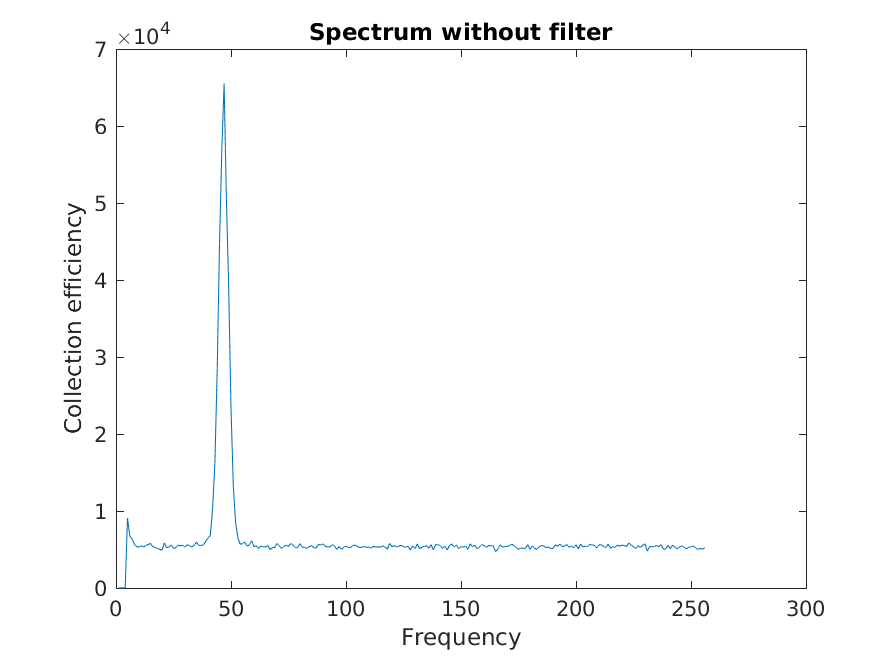
\includegraphics[width=1\linewidth]{../Exercises_and_Tasks/ex1/figures/spectra_nofilter.png}
  \caption{Raw spectrum}
  \label{fig:raw_spectrum}
\end{subfigure}
\begin{subfigure}{0.5\textwidth}
  \centering
  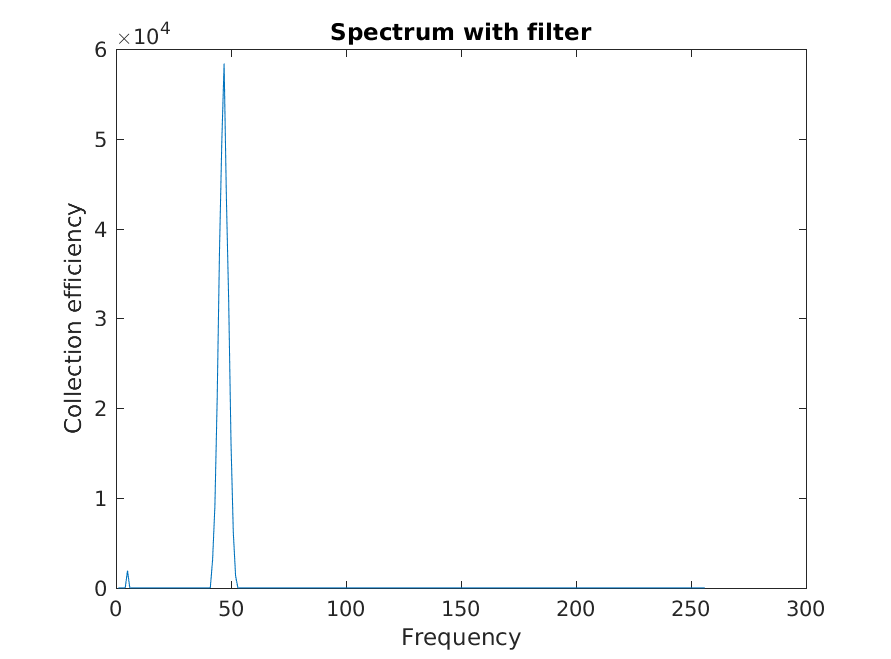
\includegraphics[width=1\linewidth]{../Exercises_and_Tasks/ex1/figures/spectra_noisecancelled.png}
  \caption{Spectrum cleaned from background noise}
    \label{fig:cleaned_spectrum}
\end{subfigure}
\end{figure}

\subsection{Calculate the Doppler frequency that each bin of the spectra corresponds to}
We received the spectra as histograms which are separated in 256 bins. The measured bandwith is $25\cdot10^6 $ Hz. Therefore each bin represents a frequency of
\begin{equation*}
 frequency = x * \frac{25\cdot10^6 Hz}{256}
\end{equation*}
where x is the bin number.
With the equations provided during the lecture we were also able to calculate the line-of-sight velocity.
The implementation in Matlab is shown in the following.\\

\begin{lstlisting}
for bin=1:256
    f_d(bin,1) = (bin-1)/bins*bandwith;
    v(bin,1) = f_d(bin,1) *lambda_0;
end;
\end{lstlisting}

\subsection{For each spectrum, define the peak location with the centroid
method}
The centroid method was introduced during the lecture and is defined as:
\begin{equation*}
f_{peak} = \frac{\int f_d \cdot p(f) df}{\int p(f) df}
\end{equation*}
Before we calculated the peak values we normalized our data to get a PDF instead of absolute values.
Since we are dealing with discrete values, we summed over all values in order to identify the peak value. 
In order to check all 312 $f_{peak}$ values, we first calculated the index of the maximum collection efficiency for each spectra. The maximum should always represent the peak of the spectrum.
Next we determined the corresponding index of $f_{peak}$. Now we were able to compare the distance of the calculated indices. The results are shown in figure \ref{fig:failures}.

\begin{figure}[H]
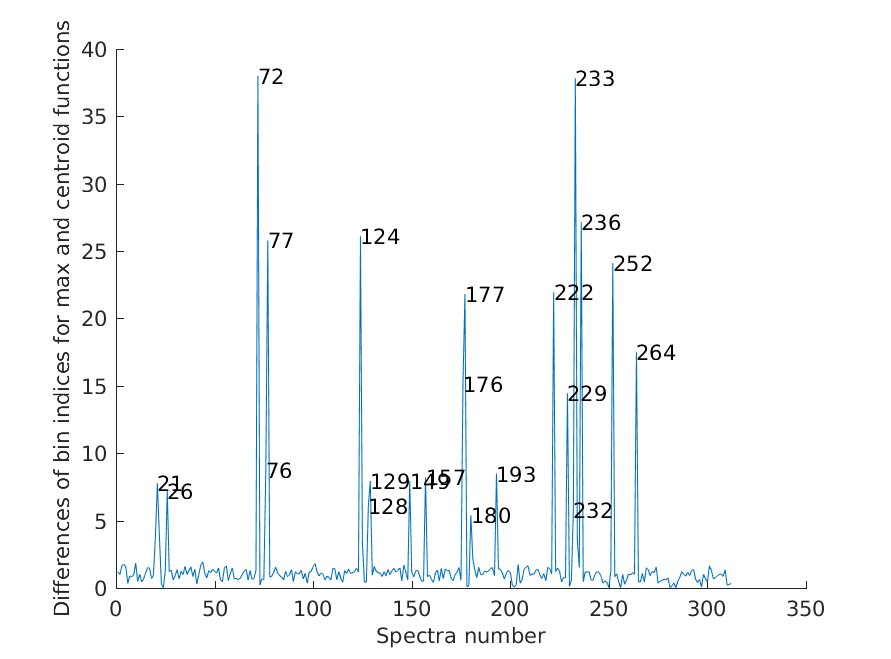
\includegraphics[width=1\linewidth]{../Exercises_and_Tasks/ex1/figures/failures.png}
\caption{Centroid Errors in bin distance}
\label{fig:failures}
\end{figure}

The figure shows that there are several errors. The reason why the centroid method fails for some spectra is due to a measurement error. As stated in the exercise sheet the lidar was placed on the nacelle of a wind turbine. Therefore for some measurements the lidar might be blocked by the rotating blades which would result in a second frequency peak. If the spectrum contains two peaks, the centroid method returns the middle of these two peaks and is not applicable for this case.
One of those cases is shown in figure \ref{fig:measurement_error}.

\begin{figure}[H]
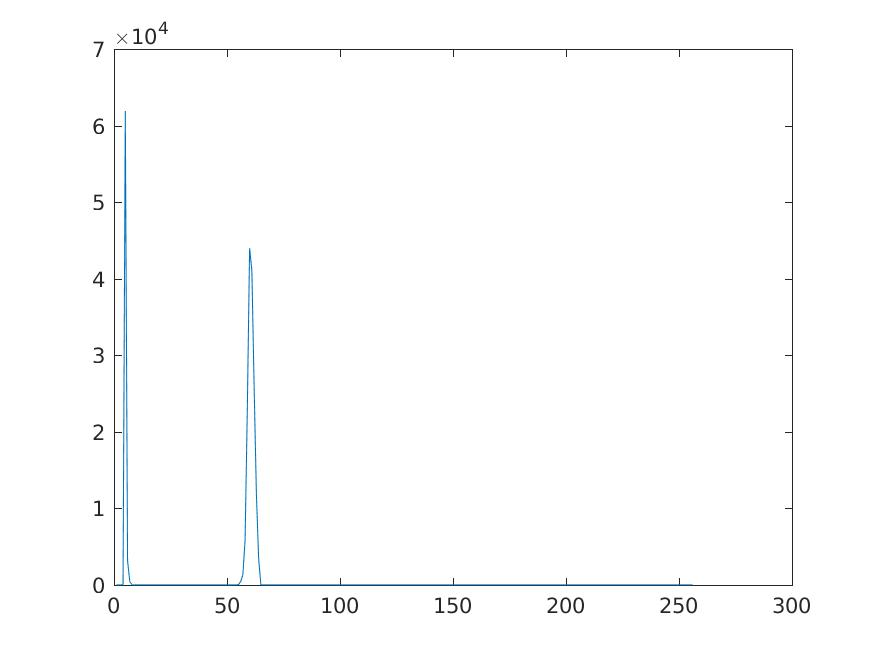
\includegraphics[width=1\linewidth]{../Exercises_and_Tasks/ex1/figures/spectra_noisecancels_normed_72.jpg}
\caption{Measurement error in spectrum 72}
\label{fig:measurement_error}
\end{figure}

\subsection{Correlate your calculated line-of-sight speeds}
In step 4 we were asked to correlate the calculated line-of-sight speeds with the lidar data itself. The correlation method was already provided. Therefore we only needed to calculate the line-of-sight velocity by multiplying $f_{peak}$ with $\lambda_0$. The resulting plot is shown in figure \ref{fig:correlation}. 

\begin{figure}[H]
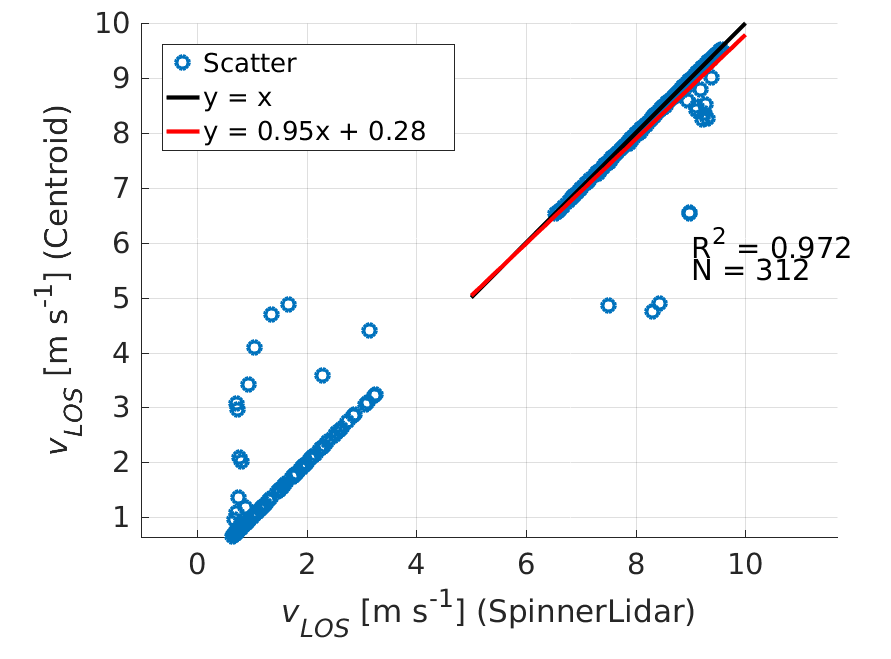
\includegraphics[width=1\linewidth]{../Exercises_and_Tasks/ex1/figures/correlation.png}
\caption{Correlation of the calculated line-of sight-speed and the lidar data}
\label{fig:correlation}
\end{figure}

Figure \ref{fig:correlation} shows a strong correlation of $R^2 = 0.972$. As discussed in section 1.3 there are measurement errors due to the position of the lidar. Some measurements are blocked by the moving blades. 

\end{document}